\documentclass[12pt]{article}
\usepackage[margin=1in]{geometry}
\usepackage[pdftex]{hyperref}
\usepackage{amsmath}
\usepackage{tikz}
\usepackage{pgfplots}
\usepackage{float}

\author{Christopher Mertin}
\title{Distributed Barnes-Hut Algorithm: Planet Simulation}

\begin{document}
\begin{titlepage}
\maketitle
\thispagestyle{empty}
\end{titlepage}

\section*{Introduction}
The N-body problem is important for many aspects of physics and scientific simulations. This is due to the fact that each particle interacts with every other type of particle, which results in an $\mathcal{O}\left( n^{2}\right)$ algorithm if you take the na\"{i}ve approach.

There are alternative ways to approach these types of problems, one of which is known as the {\em Barnes-Hut Algorithm} \cite{barneshut}. While the original algorithm was sequential, modern day methods have parallelized this approach to be used with MPI for use in clusters.

The problem with parallelizing this sort of algorithm is that it is difficult to build the tree efficiently in parallel. This was accomplished with the use of {\sc Dendro}. The actual force calculations themselves are embarassingly parallel as the position update has no dependencies. 

\section*{Numerical Calculations}
The gravitational force on one planet by another is given by

\begin{align}
\vec{F} &= G\frac{m_{1}m_{2}}{r^{2}}\hat{r}
\intertext{we also know from Newton's laws that}
\vec{F} &= m\vec{a}\label{eq:newton}
\end{align}

from these above two equations, we can figure out the force on a given planet by first calculating the force on it, and then the direction of the acceleration. This can be accomplished with something trivial such as the {\em forward-euler method} or some other basic time-stepping scheme. However, methods such as the forward-euler method perform horribly at conserving energy of the system.

However, we can use another numerical method to achieve $\mathcal{O}\left(\Delta t^{3}\right)$ accuracy, and is much better in conserving energy, with a method known as the {\em Hermite Scheme}. Something such as Runge-Kutta-4 can give $\mathcal{O}\left(\Delta t^{4}\right)$ accuracy, but does take longer. As this is a simple test case, and the function itself was made modular in the code, the Hermite algorithm was chosen. This hermite algorithm was adapted from~\cite{code}.

As we know from Equation~(\ref{eq:newton}), the acceleration is the second derivative of the position. The Hermite algorithm takes this further and calculates the {\em jerk} of the system, which is the time derivative of the acceleration. With this, we can get the position in the following order

\begin{align}
\frac{\text{d}^{2}\vec{r}_{i}}{\text{d}t^{2}} = \vec{a}_{i} &= G \sum_{\substack{j=1\\j\neq i}}^{N}\frac{m_{j}}{\left| \vec{r}_{j} - \vec{r}_{i} \right|^{3}}\left(\vec{r}_{j} - \vec{r}_{i}\right)\\
\frac{\text{d}^{3}\vec{r}_{i}}{\text{d}t^{3}} = \vec{j}_{i} &= G \sum_{\substack{j=1\\j\neq i}}^{N}m_{j}\left[ \frac{\vec{v}_{j}-\vec{v}_{i}}{\left| \vec{r}_{j} - \vec{r}_{i} \right|^{3}} - 3\frac{(\vec{r}_{j}-\vec{r}_{i})\cdot (\vec{v}_{j} - \vec{v}_{i})}{\left| \vec{r}_{j} - \vec{r}_{i} \right|^{5}}(\vec{r}_{j} - \vec{r}_{i}) \right]\\
\frac{\text{d}\vec{r}_{i}}{\text{d}t} = \vec{v}_{i}^{(n+1)} &= \vec{v}_{i}^{(n)} + \frac{1}{2}\left(\vec{a}_{i}^{(n)} + \vec{a}_{i}^{(n+1)}\right)\Delta t + \frac{1}{12}\left(\vec{j}_{i}^{(n)} - \vec{j}_{i}^{(n+1)}\right)\Delta t^{2}\label{eq:vel}\\
\vec{r}_{i}^{(n+1)} &= \vec{r}_{i}^{(n)} + \frac{1}{2}\left(\vec{v}_{i}^{(n)} + \vec{v}_{i}^{(n+1)}\right)\Delta t + \frac{1}{12}\left(\vec{a}_{i}^{(n)} - \vec{a}_{i}^{(n+1)}\right)\Delta t^{2}\label{eq:pos}
\end{align}

So first the jerk and accleration need to be calculated, and then the velocity, followed by the position being updated. This needs to be done for each of the particles to have the desired result. The exponents in Equation~(\ref{eq:vel}) and Equation~(\ref{eq:pos}) denote the time step. $(n+1)$ is for the {\em new} time step, while $(n)$ is for the previous time step, and the subscript $i$ denoting the $i^{th}$ planet.

\subsubsection*{Verifying Numerical Results}
It was quite easy to verify to make sure the code was performing correctly. For the code to perform correctly, the {\em total energy} of the system had to be conserved as there were no outside forces. This relied on the {\em potential energy} and the {\em kinetic energy} of the system. 

The potential energy $(U)$ can be calculated as

\begin{align*}
U &= -G\frac{m_{1}m_{2}}{\left| \vec{r}_{2} - \vec{r}_{1}\right|}
\intertext{with $G$ being the gravitational constant, $m_{i}$ being the mass for the two planets, and $\vec{r}$ being their position. The kinetic energy $(T)$ can be represented as}
T &= \frac{1}{2}m\left| \vec{v}\right| ^{2}\\
\intertext{where $v$ is the velocity of a planet. In 3D, this is transformed into}
T &= \frac{1}{2}M\left(v_{x}^{2} + v_{y}^{2} + v_{z}^{2}\right)
\end{align*}

The total energy of the system can be computed as $U + T$ at the start of the simulation, and again after the final time step. The total energy of the system should be conserved within some percent error.

For all the different tests, the error remained within 2\% error for any number of iterations. This is well within the bounds of the simulation and can be treated as correct. This error comes about from the approximation resulting in the Barnes-Hut algorithm.

\section*{Barnes-Hut Algorithm}
The Barnes-Hut algorithm works by using an adaptive quadtree, which is shown in Figure~\ref{fig:sep}. In this figure, each color represents one ``branch'' of the quadtree. The blue branch is refined more than the others due to the point located in it. It is known as an {\em adaptive quadtree} because it only refines the grid up to the point where particles can be approximated reasonably well as a single particle.

\begin{figure}[H]
\centering
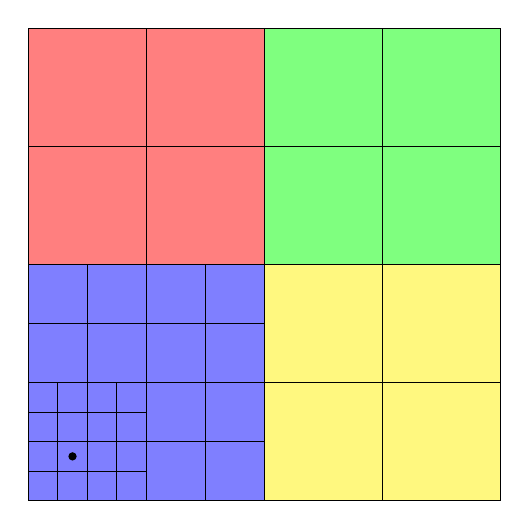
\begin{tikzpicture}[scale=.75]
\draw (0,0) -- (8,0) -- (8,8) -- (0,8) -- (0,0);
\filldraw[fill=green, draw=black, fill opacity=0.5] (4,4) rectangle (8,8);
\filldraw[fill=red, draw=black, fill opacity=0.5] (0,4) rectangle (4,8);
\filldraw[fill=yellow, draw=black, fill opacity=0.5] (4,0) rectangle (8,4);
\filldraw[fill=blue, draw=black, fill opacity=0.5] (0,0) rectangle (4,4);
\draw (2,0) -- (2,8);
\draw (6,0) -- (6,8);
\draw (0,2) -- (8,2);
\draw (0,6) -- (8,6);
\draw (1,0) -- (1,4);
\draw (3,0) -- (3,4);
\draw (0,1) -- (4,1);
\draw (0,3) -- (4,3);
\draw (.5,0) -- (.5,2);
\draw (1.5,0) -- (1.5,2);
\draw (0,.5) -- (2,.5);
\draw (0,1.5) -- (2,1.5);
\fill (.75,.75) circle (2pt);
\end{tikzpicture}
\caption{Adaptive Quadtree}
\label{fig:sep}
\end{figure}

To approximate the single particle, the center of mass is calculated for all the particles in that octant. The total mass in that octant would be the sum of the masses. In other words:

\begin{align}
\vec{r}_{i} = \frac{\sum_{i=1}^{\zeta}m_{i}\vec{x}_{i}}{\sum_{i=1}^{\zeta}m_{i}}
\end{align}

where $\zeta$ is the total number of particles in the given octant. This new position and mass are used to approximate the particles that are reasonably far enough away to be approximated as a single point.

The colors in Figure~\ref{fig:quadtree} represent those particles that are ``far enough away.'' Those in red are approximated as larger particles, and they decrease in size as you go down to finer grains. The larger the particles in the grid, the more that were approximated/averaged in that octant. The ones in the yellow grid are down to the finest grain size where each dot represents a single particle. The finest octant size is given for those in yellow, which are the octant's neighbors. 

\begin{figure}[H]
\centering
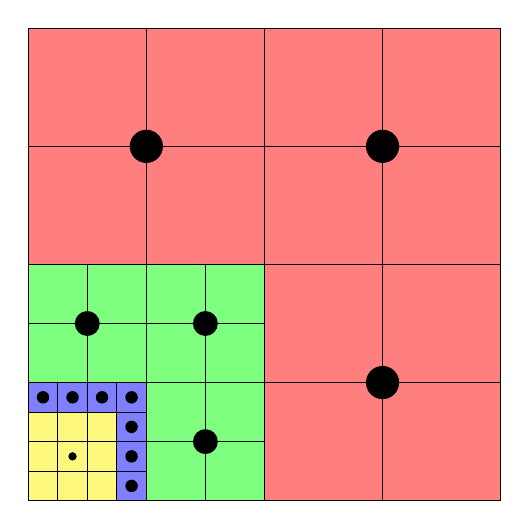
\begin{tikzpicture}[scale=.75]
\draw (0,0) -- (8,0) -- (8,8) -- (0,8) -- (0,0);
\filldraw[fill=red, draw=black, fill opacity = .5] (0,0) rectangle (8,8);
\filldraw[fill=white, draw=black] (0,0) rectangle (4,4);
\filldraw[fill=green, draw=black, fill opacity = .5] (0,0) rectangle (4,4);
\filldraw[fill=white, draw=black] (0,0) rectangle (2,2);
\filldraw[fill=blue, draw=black, fill opacity = .5] (0,0) rectangle (2,2);
\filldraw[fill=white, draw=black] (0,0) rectangle (1.5,1.5);
\filldraw[fill=yellow, draw=black, fill opacity = .5] (0,0) rectangle (1.5,1.5);
\draw (4,0) -- (4,8);
\draw (0,4) -- (8,4);
\draw (2,0) -- (2,8);
\draw (6,0) -- (6,8);
\draw (0,2) -- (8,2);
\draw (0,6) -- (8,6);
\draw (1,0) -- (1,4);
\draw (3,0) -- (3,4);
\draw (0,1) -- (4,1);
\draw (0,3) -- (4,3);
\draw (.5,0) -- (.5,2);
\draw (1.5,0) -- (1.5,2);
\draw (0,.5) -- (2,.5);
\draw (0,1.5) -- (2,1.5);
\fill (.75,.75) circle (2pt);
\fill (2,6) circle (8pt);
\fill (6,6) circle (8pt);
\fill (6,2) circle (8pt);
\fill (1,3) circle (6pt);
\fill (3,3) circle (6pt);
\fill (3,1) circle (6pt);
\fill (1.25,1.75) circle (3pt);
\fill (.75,1.75) circle (3pt);
\fill (.25,1.75) circle (3pt);
\fill (1.75,1.75) circle (3pt);
\fill (1.75,1.25) circle (3pt);
\fill (1.75,.75) circle (3pt);
\fill (1.75,.25) circle (3pt);
\end{tikzpicture}
\caption{Adaptive Quadtree Coarsening}
\label{fig:quadtree}
\end{figure}

The code can be found \cite{github} under the github branch {\tt CS6320\_Semester\_Project}. The complexity of building the tree in {\sc Dendro} is $\mathcal{O}\left( \frac{N}{p}\log\left( N/p\right)\right)$. Since the positions of the particles are updated after each time step, the octants change as well. This can be prevented by altering/adjusting the tree after each time step. However, the implementation that was used was rebuilding the tree after each iteration. Therefore, the {\em time complexity} is $\mathcal{O}\left( t \frac{N}{p}\log\left( N/p\right)\right)$, where $t$ is the number of time steps.

{\sc Dendro} is ``probably, yea'' work-optimal \cite{milinda}. The calculation part is work optimal as it can be parallelized easily and not have to do any extra work.


\section*{Results}
The results of the implemented Barnes-Hut algorithm can be seen in Figures~\ref{fig:weak_scaling} and \ref{fig:strong_scaling}.

In Figure~\ref{fig:weak_scaling}, the large jump and irregularities in the plot are most likely due to the inefficient communication that was implemented. In the current implementation, at the start of each iteration an {\tt MPI\_Allgather} was performed so that each node/process had all the paricles so they could see which it needed for what octants. After implementing the code, it was realized that there could be an {\em interprocessor sorting} done between the nodes, removing the {\tt MPI\_Allgather} requirement. There were a few other {\tt MPI\_Allgather} and {\tt MPI\_Allreduce} commands that were performed which were realized after that they could be removed.

With more time, these could be fixed so that the code was more efficient. The code and timings were performed on {\sc Mir} since {\sc Tangent} did not have {\sc Petsc} installed and was unable to be installed locally.

The strong scaling results in Figure~\ref{fig:strong_scaling} seem to agree with how the scalability should look. The timings follow the general pattern for the time taken to solve the problem.

In order to compare the results, the sequential case for the $\mathcal{O}\left( N^{2}\right)$ algorithm was implemented and timed as well. Those timings can be seen in Table~\ref{table:sequential}. The implemented code performed {\em worse} than the $\mathcal{O}\left( N^{2}\right)$ algorithm for $p < 12$ and $N < 8000$. This is likely due to the extra requirement to build the tree with every iteration and savings not coming about except for large $N$.

%    Results: Describe the experiments you performed to evaluate your code/methods. Summarize results and discuss them. Are the results what you expected. If not, why are they better or worse then what you expected. What other experiments would you have done if you had more time. With the knowledge of the results, would you change your methods in any way to improve performance or scalability. 


\begin{figure}[H]
\centering
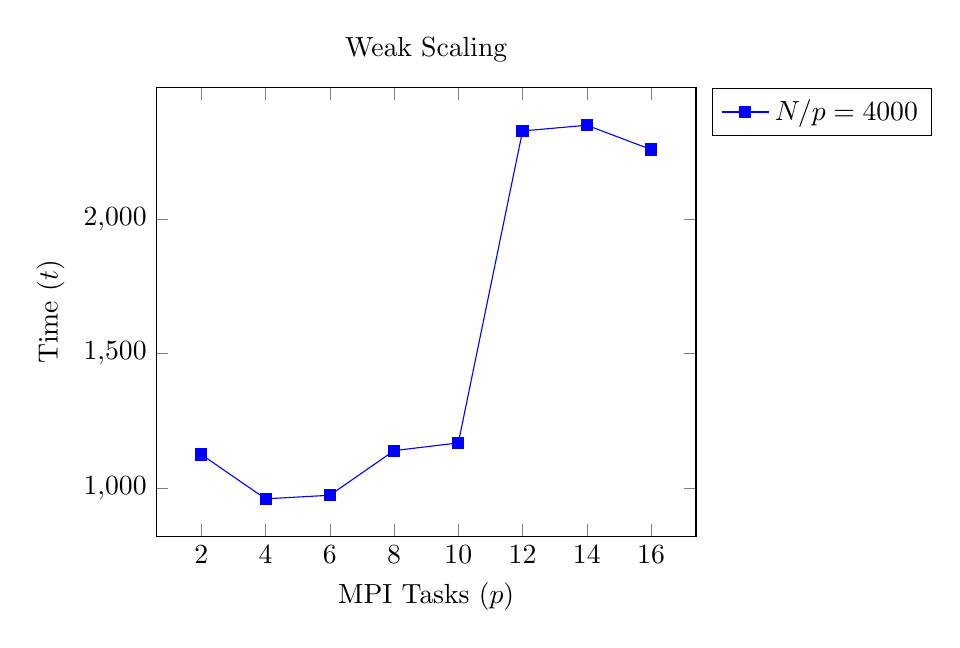
\begin{tikzpicture}
\begin{axis}[title={Weak Scaling}, xlabel={MPI Tasks $(p)$}, ylabel={Time $(t)$}, legend pos=outer north east]
\addplot[color=blue, mark=square*,]coordinates{(2, 1124.41)(4, 959.32)(6,972.64)(8,1138.98)(10,1167.73)(12,2330.16)(14,2351.48)(16,2260.98)};
\legend{$N/p=4000$}
\end{axis}
\end{tikzpicture}
\caption{$N/p$ remains constant}
\label{fig:weak_scaling}
\end{figure}

\begin{figure}[H]
\centering
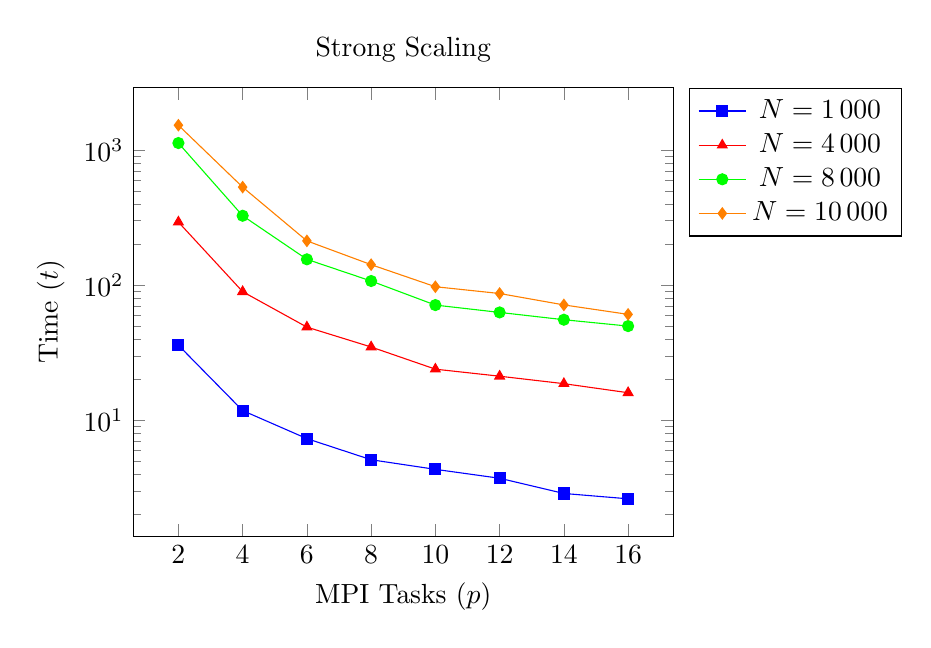
\begin{tikzpicture}
\begin{axis}[title={Strong Scaling}, xlabel={MPI Tasks $(p)$}, ylabel={Time $(t)$}, ymode=log, legend pos=outer north east]
\addplot[color=blue, mark=square*]coordinates{(2,35.93)(4,11.79)(6,7.31)(8,5.10)(10,4.33)(12,3.72)(14,2.87)(16,2.62)};
\addplot[color=red, mark=triangle*]coordinates{(2,293.31)(4,89.53)(6,48.94)(8,34.87)(10,23.89)(12,21.19)(14,18.66)(16,15.99)};
\addplot[color=green, mark=*]coordinates{(2,1128.71)(4,326.75)(6,155.42)(8,107.37)(10,71.25)(12,62.87)(14,55.51)(16,49.80)};
\addplot[color=orange, mark=diamond*]coordinates{(2,1529.18)(4,532.14)(6,212.84)(8,141.9024)(10,97.43)(12,86.79)(14,71.45)(16,60.82)};
\legend{$N = 1\,000$, $N = 4\,000$, $N = 8\,000$, $N = 10\,000$}
\end{axis}
\end{tikzpicture}
\caption{$N$ remains constant}
\label{fig:strong_scaling}
\end{figure}

\begin{table}[H]
\centering
\caption{Timings for Sequential}
\begin{tabular}{@{}l | r@{}}
\hline\hline
$N$ & $t$\\
\hline
1000 & 1.04\\
4000 & 16.61\\
8000 & 66.07\\
10000 & 103.11\\
\hline
\end{tabular}
\label{table:sequential}
\end{table}


%\subsubsection*{Future Work}

\begin{thebibliography}{99}
\bibitem{barneshut}Josh Barnes and Piet Hut, {\em A Hierarchial $\mathcal{O}\left( N\log(N)\right)$ Force-Calculation Algorithm}, Nature {\bf 324} (4), (December 1986) 446-449
\bibitem{code} Piet Hut and Jun Makino, {\em Moving Stars Around}, \url{http://www.artcompsci.org/}
\bibitem{github}\textit{Barnes-Hut: \textsc{Dendro}}, \url{https://github.com/cmertin/dendro}
\bibitem{milinda} Weerahannadige Milinda Shayamal Fernando, Personal Conversation, May 9, 2016
\end{thebibliography}
\end{document}